\documentclass[lang=cn]{elegantpaper}

\title{行车灯光}

\begin{document}

\maketitle

本题目中状态机直接并没有直接的关系,而是直接由输入决定,当前的直行和下一时刻的转弯并无直接联系。因此本作业采用了组合逻辑完成了状态的定义,在不同的状态内部通过计数的方式完成状态的循环\footnote{这才是某种意义上存在状态转移的状态机。} 。

关于计数,本次作业很贴心的采取了二的幂次的循环长度,因此可以直接自增,通过有意识的溢出完成复位。

而作者也曾尝试使用 \lstinline{task} 的方式实现切换特定的输出的功能但是放弃了,关于这部分会在下一实验详细叙述,而这也是简化的代码的一大利器。

关于输入导致状态的切换不能立即产生对灯光影响的问题,其实可以通过将其转换为一个巨大无比的 Mealy状态机 实现,但是这样会造成大量的硬件浪费,而一到二个周期的延迟应该被视作可以接受的。

波形由于序列过长,因此请参阅 \lstinline{test.vcd, test.wlf } 。仅展示一部分状态。


\begin{figure}[htb]
    \centering
    \caption{紧急状态}\label{01}
    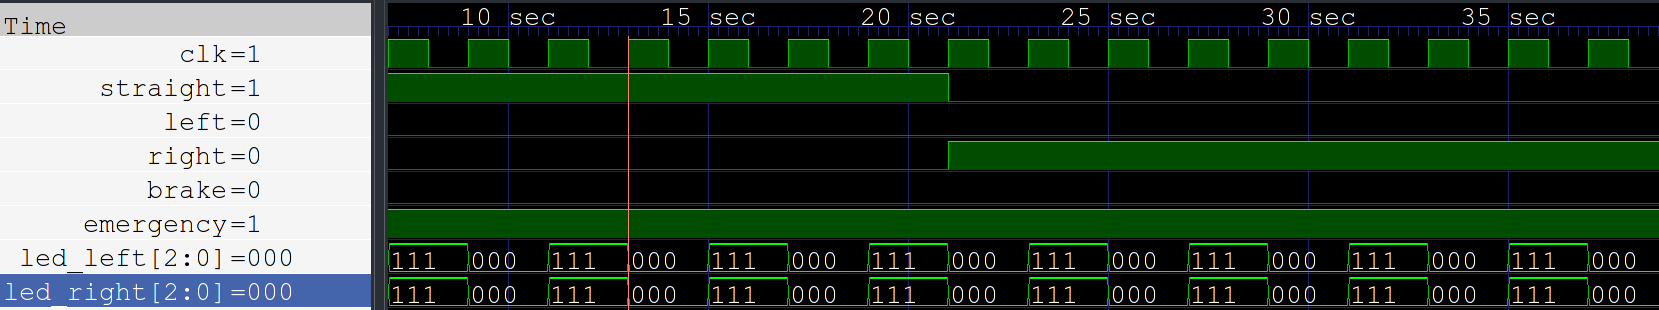
\includegraphics[width=0.6\textwidth]{eme.png}
\end{figure}


\begin{figure}[htb]
    \centering
    \caption{刹车}\label{02}
    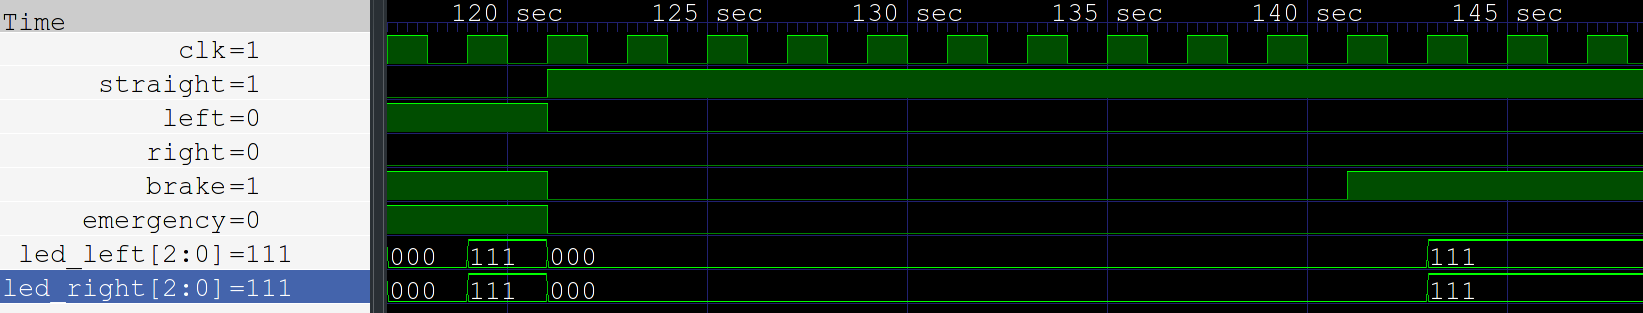
\includegraphics[width=0.6\textwidth]{brake.png}
\end{figure}


\begin{figure}[htb]
    \centering
    \caption{左侧刹车}\label{03}
    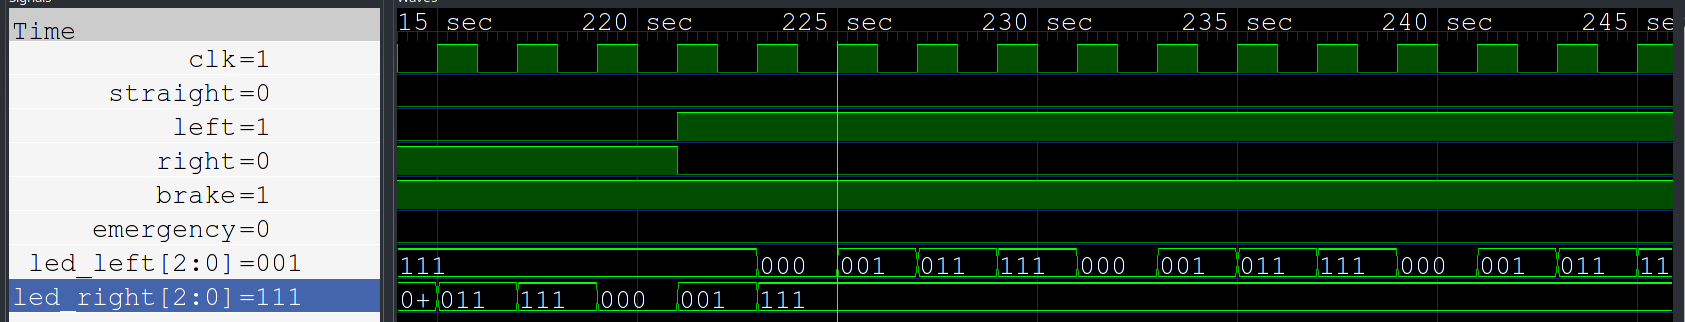
\includegraphics[width=0.6\textwidth]{leftb.png}
\end{figure}


\end{document}